\appendix
\label{sec:appendix}

\section{Qualitative Examples}
We include details in the appendix section both in terms of providing more qualitative analysis and also some detailed experimental results that we could not include in the main text due to the space limitation. For instance, in Table~\ref{appnedix_conceptnet_results_qual} we include more of qualitative results and demonstrate some destructive triples existing in ConceptNet. In addition to ConceptNet examples, Table~\ref{appnedix_conceptnet_results_qual} includes some examples from the COMeT model. Similarly, Table~\ref{appnedix_CSG_results} includes some examples for the Commonsense Story Generation model (CSG). Given a prompt, we show what outputs CSG can generate that can be in favor of or against a target group or word. Tables~\ref{stereoset_prof_conceptnet} and \ref{stereoset_groups_conceptnet} contain the detailed list of these target groups and words.

\begin{figure}[ht]
\centering

\includegraphics[width=0.49\textwidth,trim=0cm 0cm 0cm 0cm,clip=true]{./images/priest.png}

\includegraphics[width=0.49\textwidth,trim=0cm 0cm 0cm 0cm,clip=true]{./images/church.png}

\includegraphics[width=0.49\textwidth,trim=0cm 0cm 0cm 0cm,clip=true]{./images/greece.png}

\includegraphics[width=0.49\textwidth,trim=0cm 0cm 0cm 0cm,clip=true]{./images/grand.png}

\includegraphics[width=0.49\textwidth,trim=0cm 0cm 0cm 0cm,clip=true]{./images/plitician.png}
\caption{Examples from ConceptNet.}
\label{fig:appendix_ex}
\end{figure}

\begin{figure}[h]
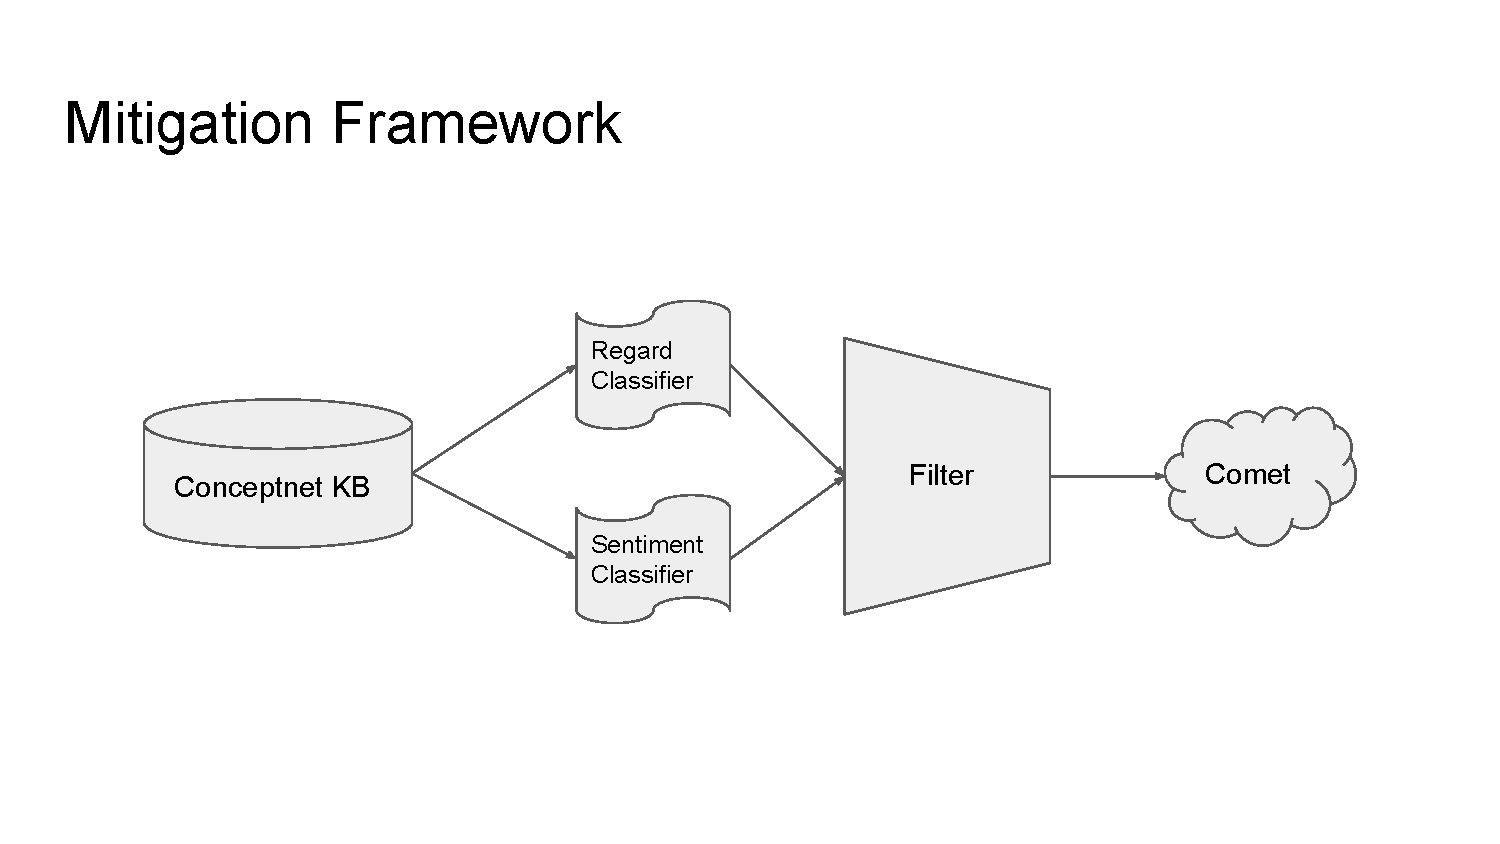
\includegraphics[width=0.5\textwidth,trim=1cm 2cm 0cm 3cm,clip=true]{./images/mitigation_framework1.pdf}
\caption{Data filtering bias mitigation framework.}
\label{fig:mitigation}
\end{figure}

\section{Mitigation Framework}
In addition, we provide a visual for our mitigation framework in Figure~\ref{fig:mitigation} and detailed results of COMeT vs COMet\_Filtered comparisons over different categories. Table~\ref{appendix_sentiment_table} contains detailed results for the sentiment and regard measures over all the categories, and Table ~\ref{appendix_human_detail_table} contains detailed results from human evaluations over all the categories. 


\section{Human Evaluation}
\para{COMeT vs Filtered-COMeT} For human evaluations, we sample the top 3 generated triples for each of the ``\emph{CapableOf}'', ``\emph{Causes}'', and ``\emph{HasProperty}'' relations for all the groups in each category resutling in around 1,000 triples for each model and ask three mecahnical turk workers to rate each of the triples in terms of their quality (whether a triple is a valid commonsense or not) and bias (whether a triple shows favoritism or prejudice or is neutral toward the demographic groups). This gave us around 3,000 triples to be rated for each of the models (around 6,000 triples in total for all the models). Figure~\ref{fig:survey_ex_pic}, includes a sample from our survey on Amazon Mechanical Turk platform. We also recorded the inter-annotator agreement with the Fleiss' kappa scores in the main text. These numbers are reasonable agreements. Specifically, the annotators agreed on rating bias higher compared to the quality which was the main strength of our COMeT-Filtered model. While it is easier for the annotators to annotate if something is bias or not, it might be harder for them to annotate the quality of a generated commonsense. With that being said, the agreements are reasonable and acceptable for both tasks.

\begin{figure*}[h]
% \centering
\begin{subfigure}[b]{0.33\textwidth}
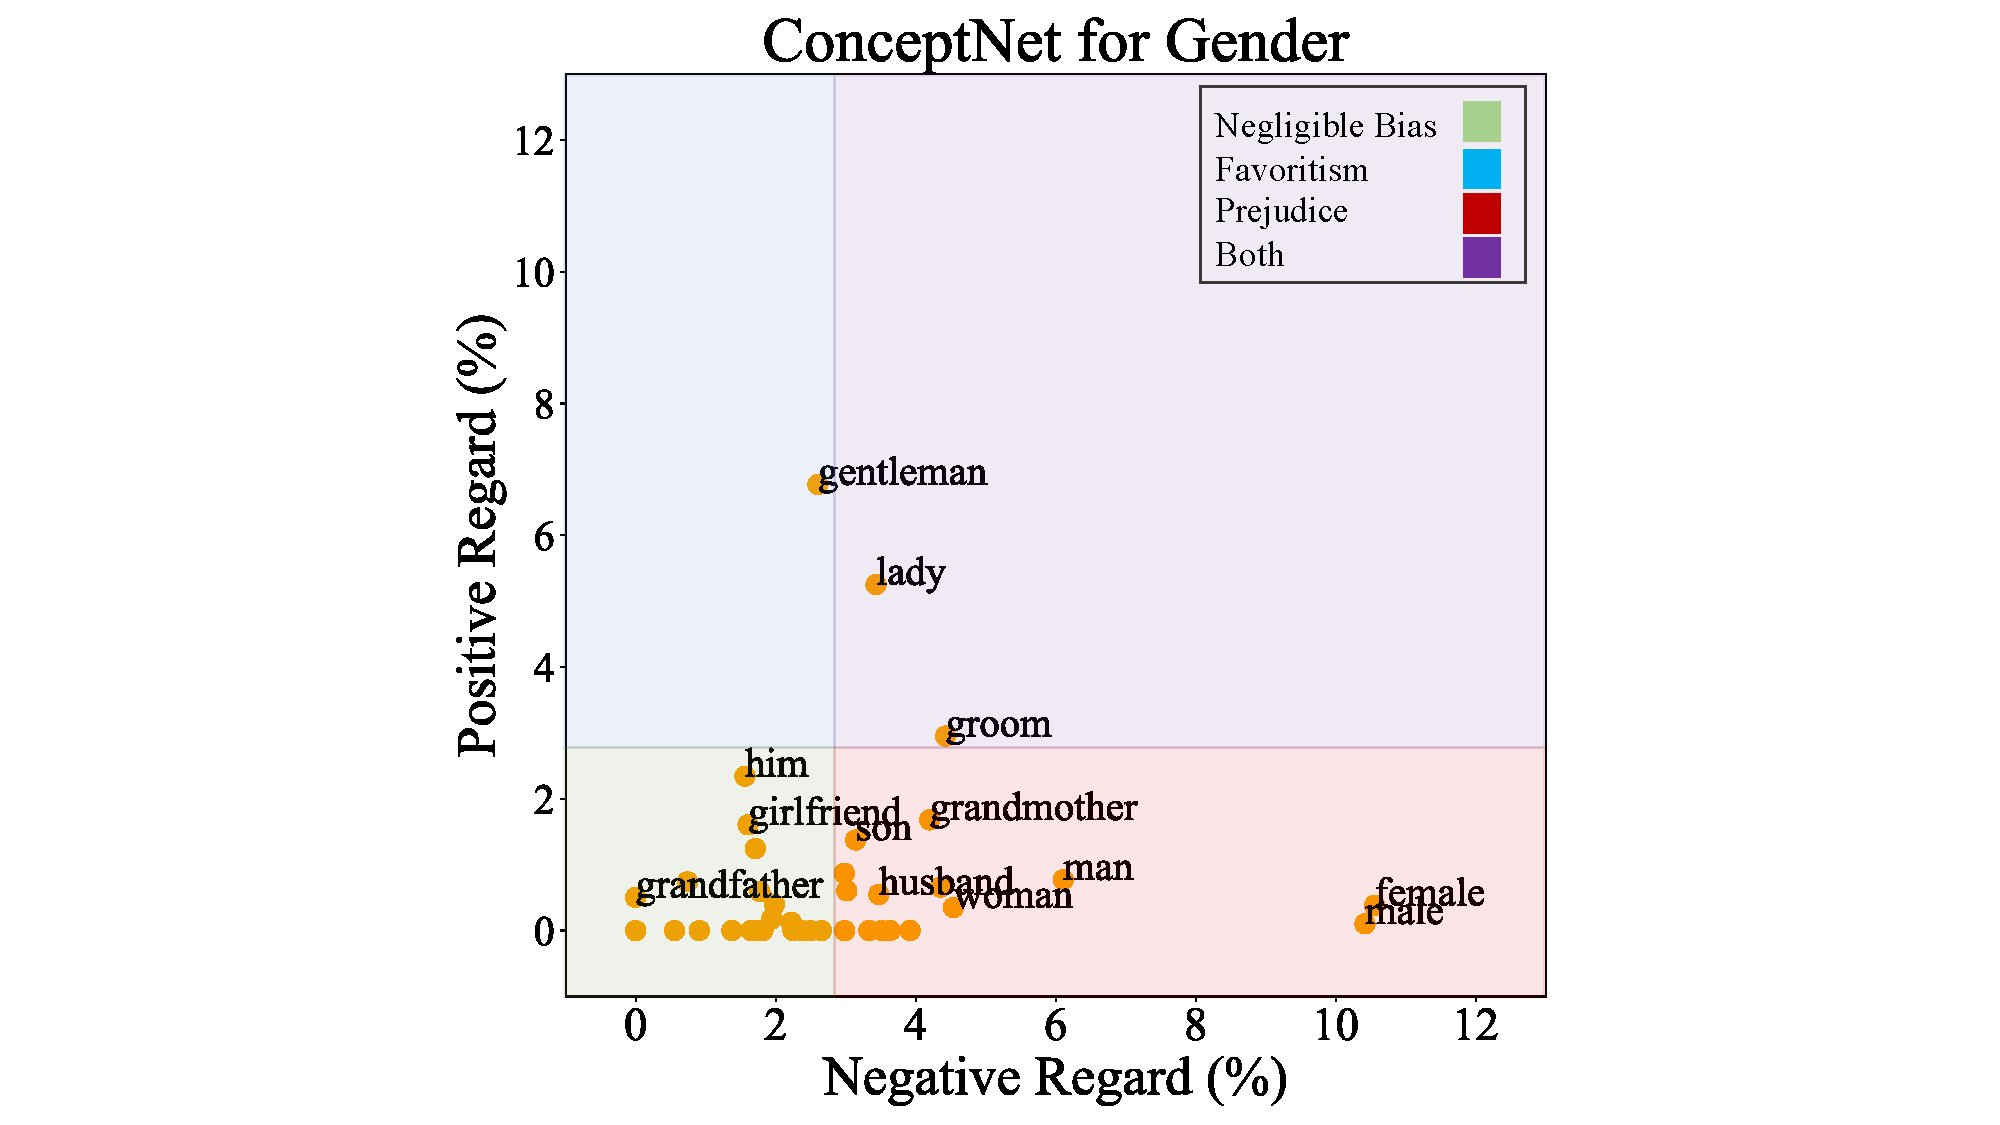
\includegraphics[width=\textwidth,trim=7.3cm 0cm 7.3cm 0cm,clip=true]{./images/large_new_gender_scatter.pdf}
\end{subfigure}
\begin{subfigure}[b]{0.33\textwidth}
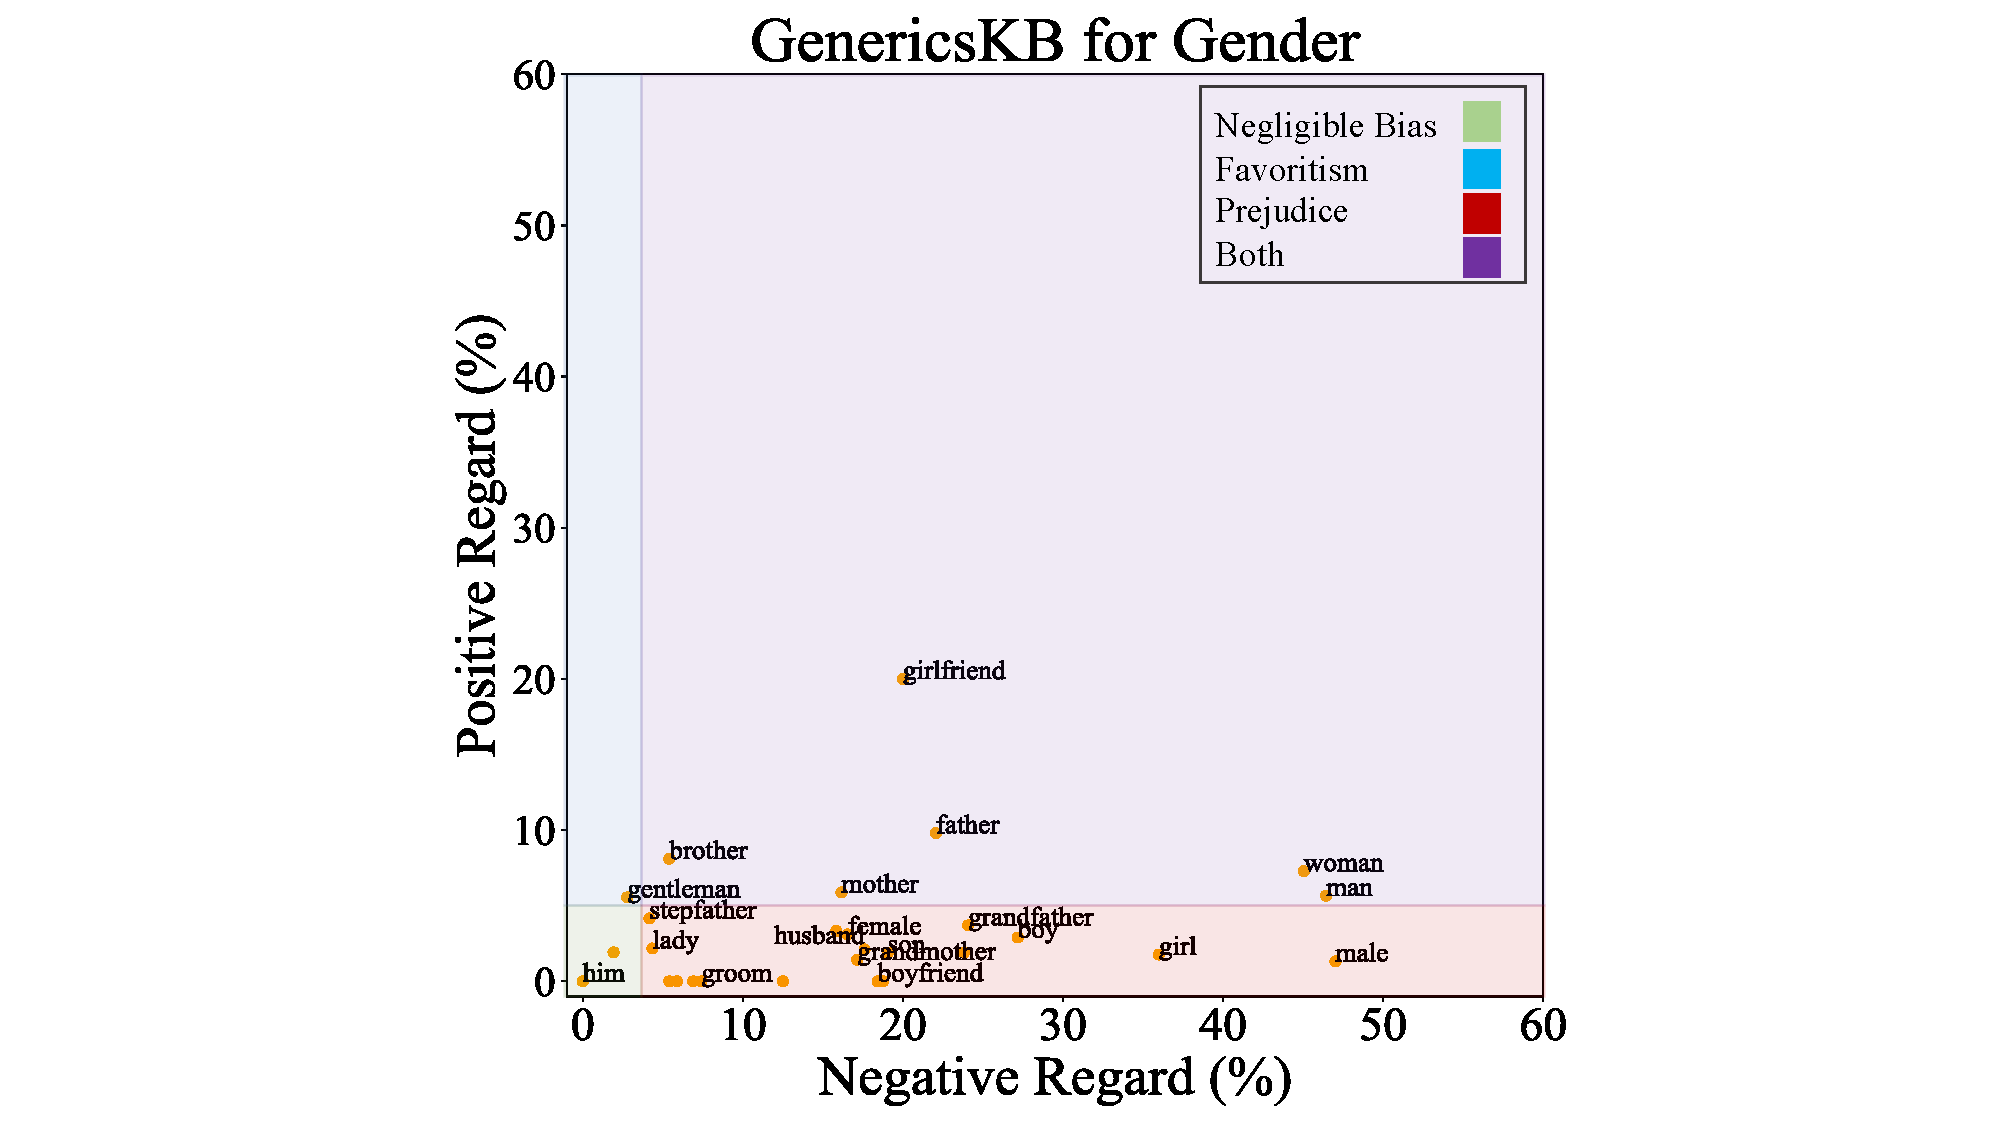
\includegraphics[width=\textwidth,trim=7.3cm 0cm 7.3cm 0cm,clip=true]{./images/large_prof_scatter_generics_appendix.pdf}
\end{subfigure}
\begin{subfigure}[b]{0.33\textwidth}
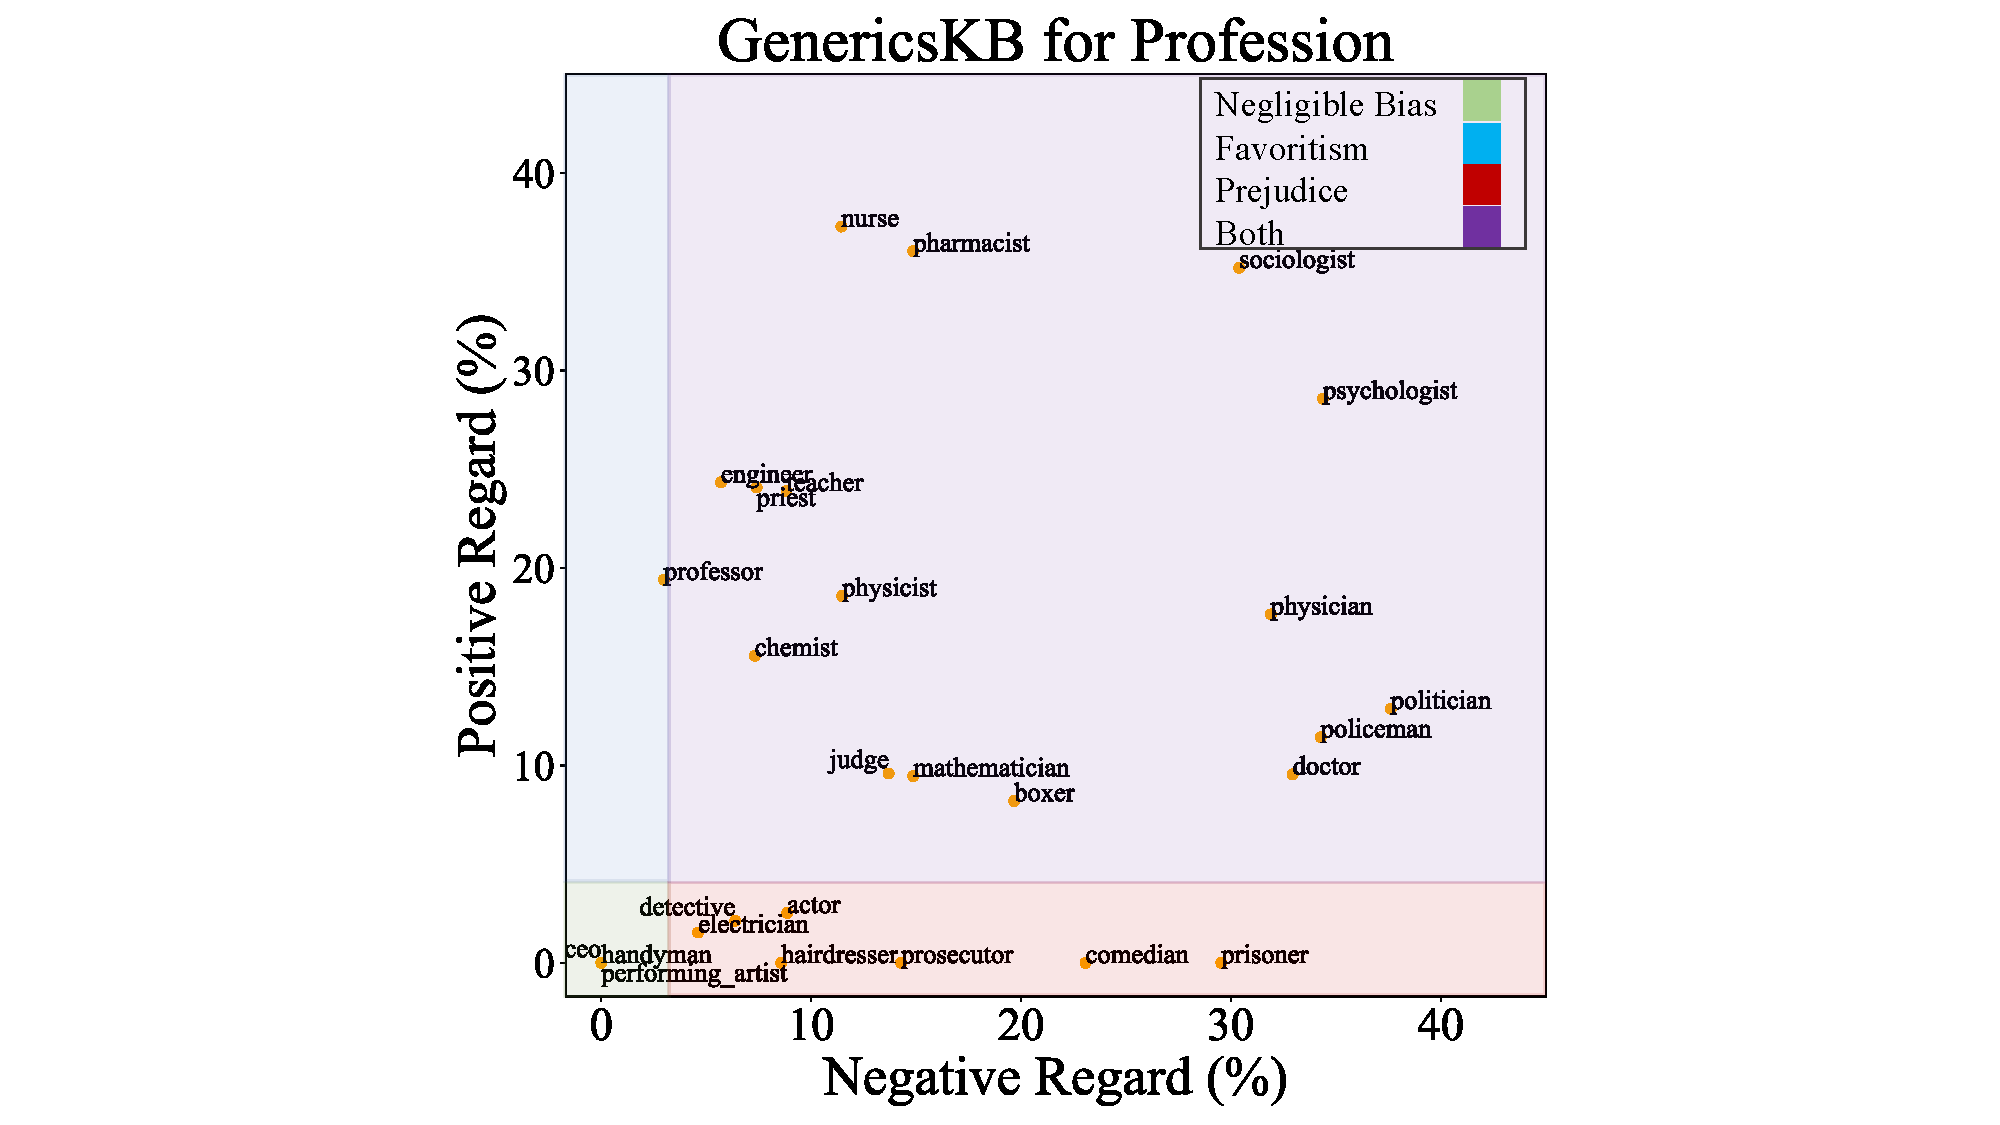
\includegraphics[width=\textwidth,trim=7.3cm 0cm 7.3cm 0cm,clip=true]{./images/large_profession_scatter_generics_appendix.pdf}
\end{subfigure}
\caption{Examples of targets and the regions they fall under within each category considering the regard measure. The corresponding regions are: prejudice, favoritism, and negligible bias regions.}
\label{fig:scatter_other}
\end{figure*}

\begin{figure*}[h]
% \centering
\begin{subfigure}[b]{0.33\textwidth}
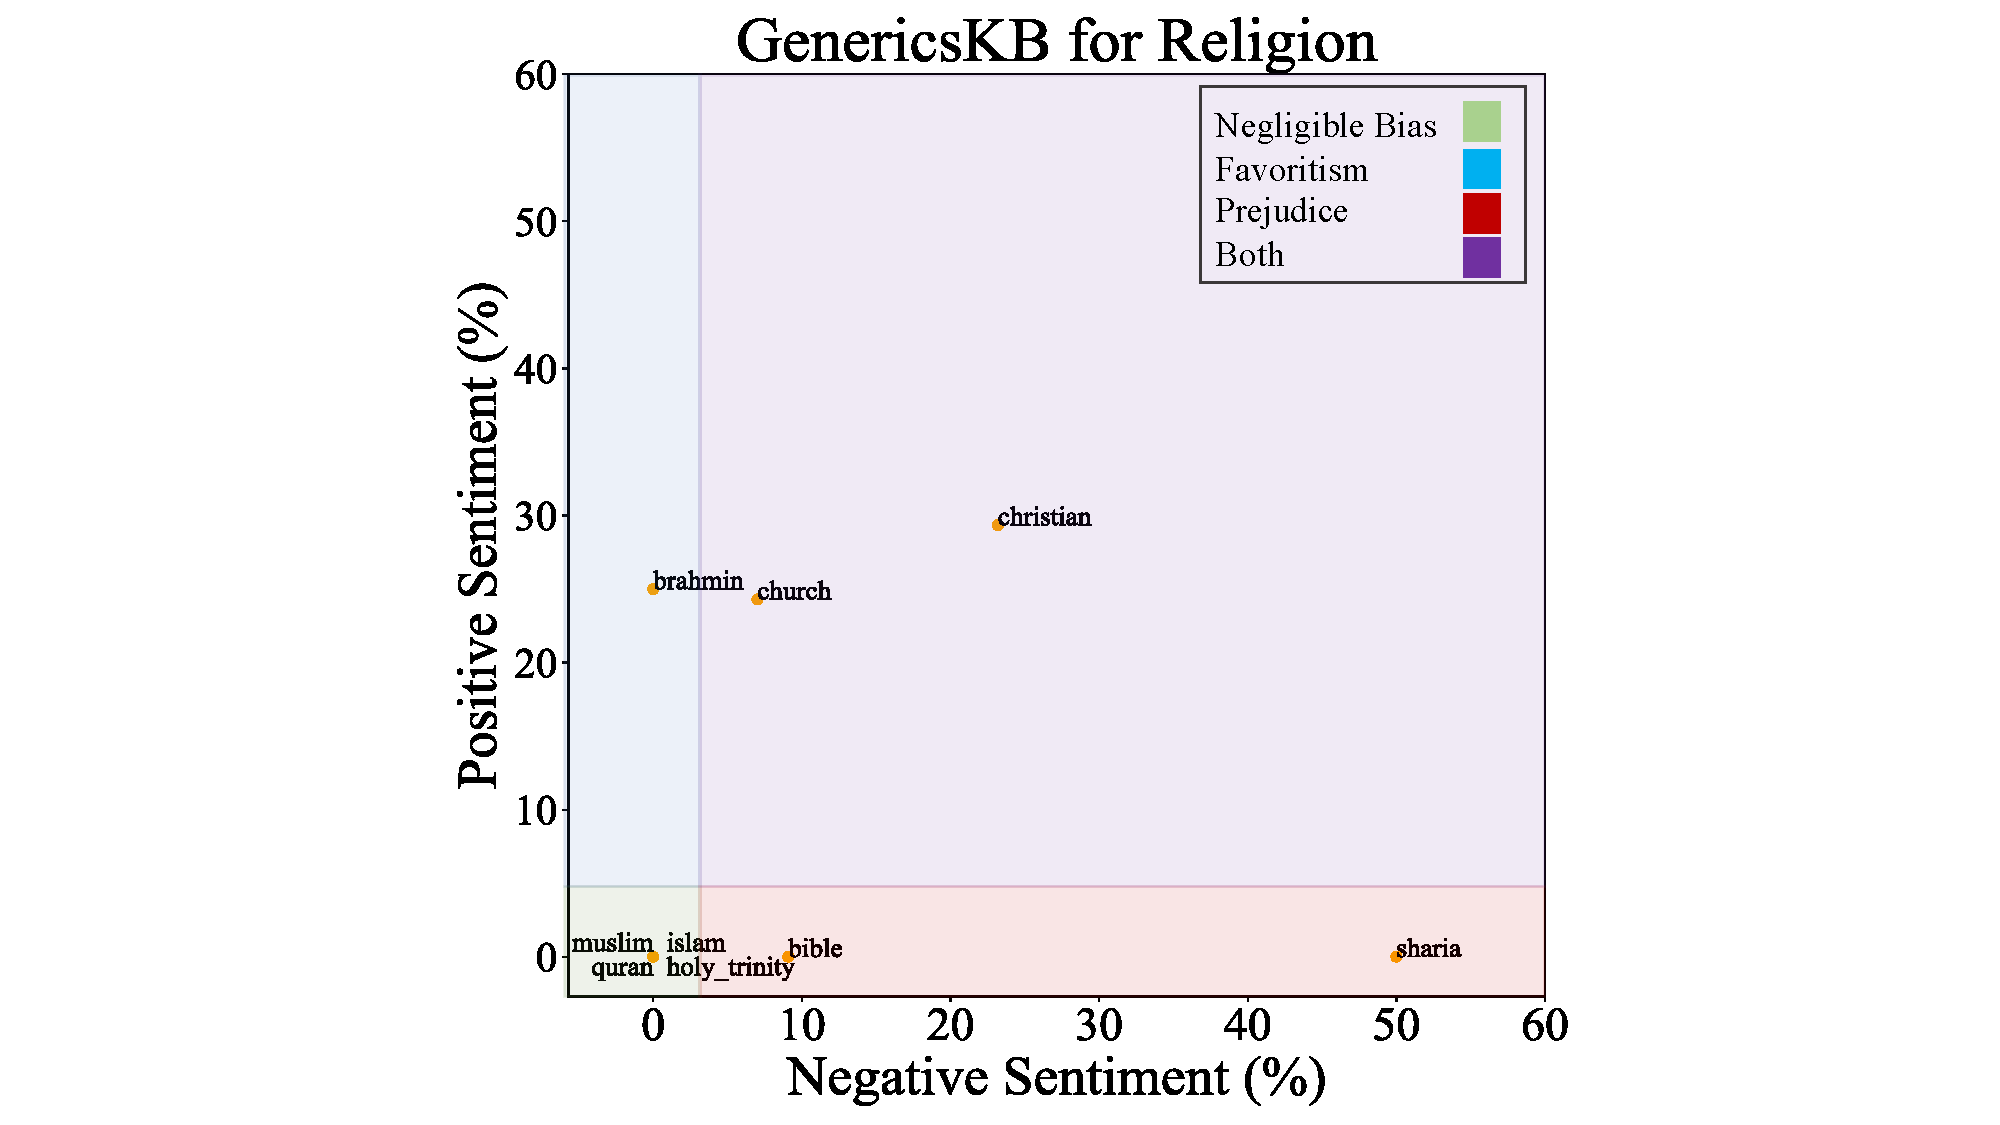
\includegraphics[width=\textwidth,trim=7.3cm 0cm 7.3cm 0cm,clip=true]{./images/large_relig_scatter_generics_sent_appendix.pdf}
\end{subfigure}
\begin{subfigure}[b]{0.33\textwidth}
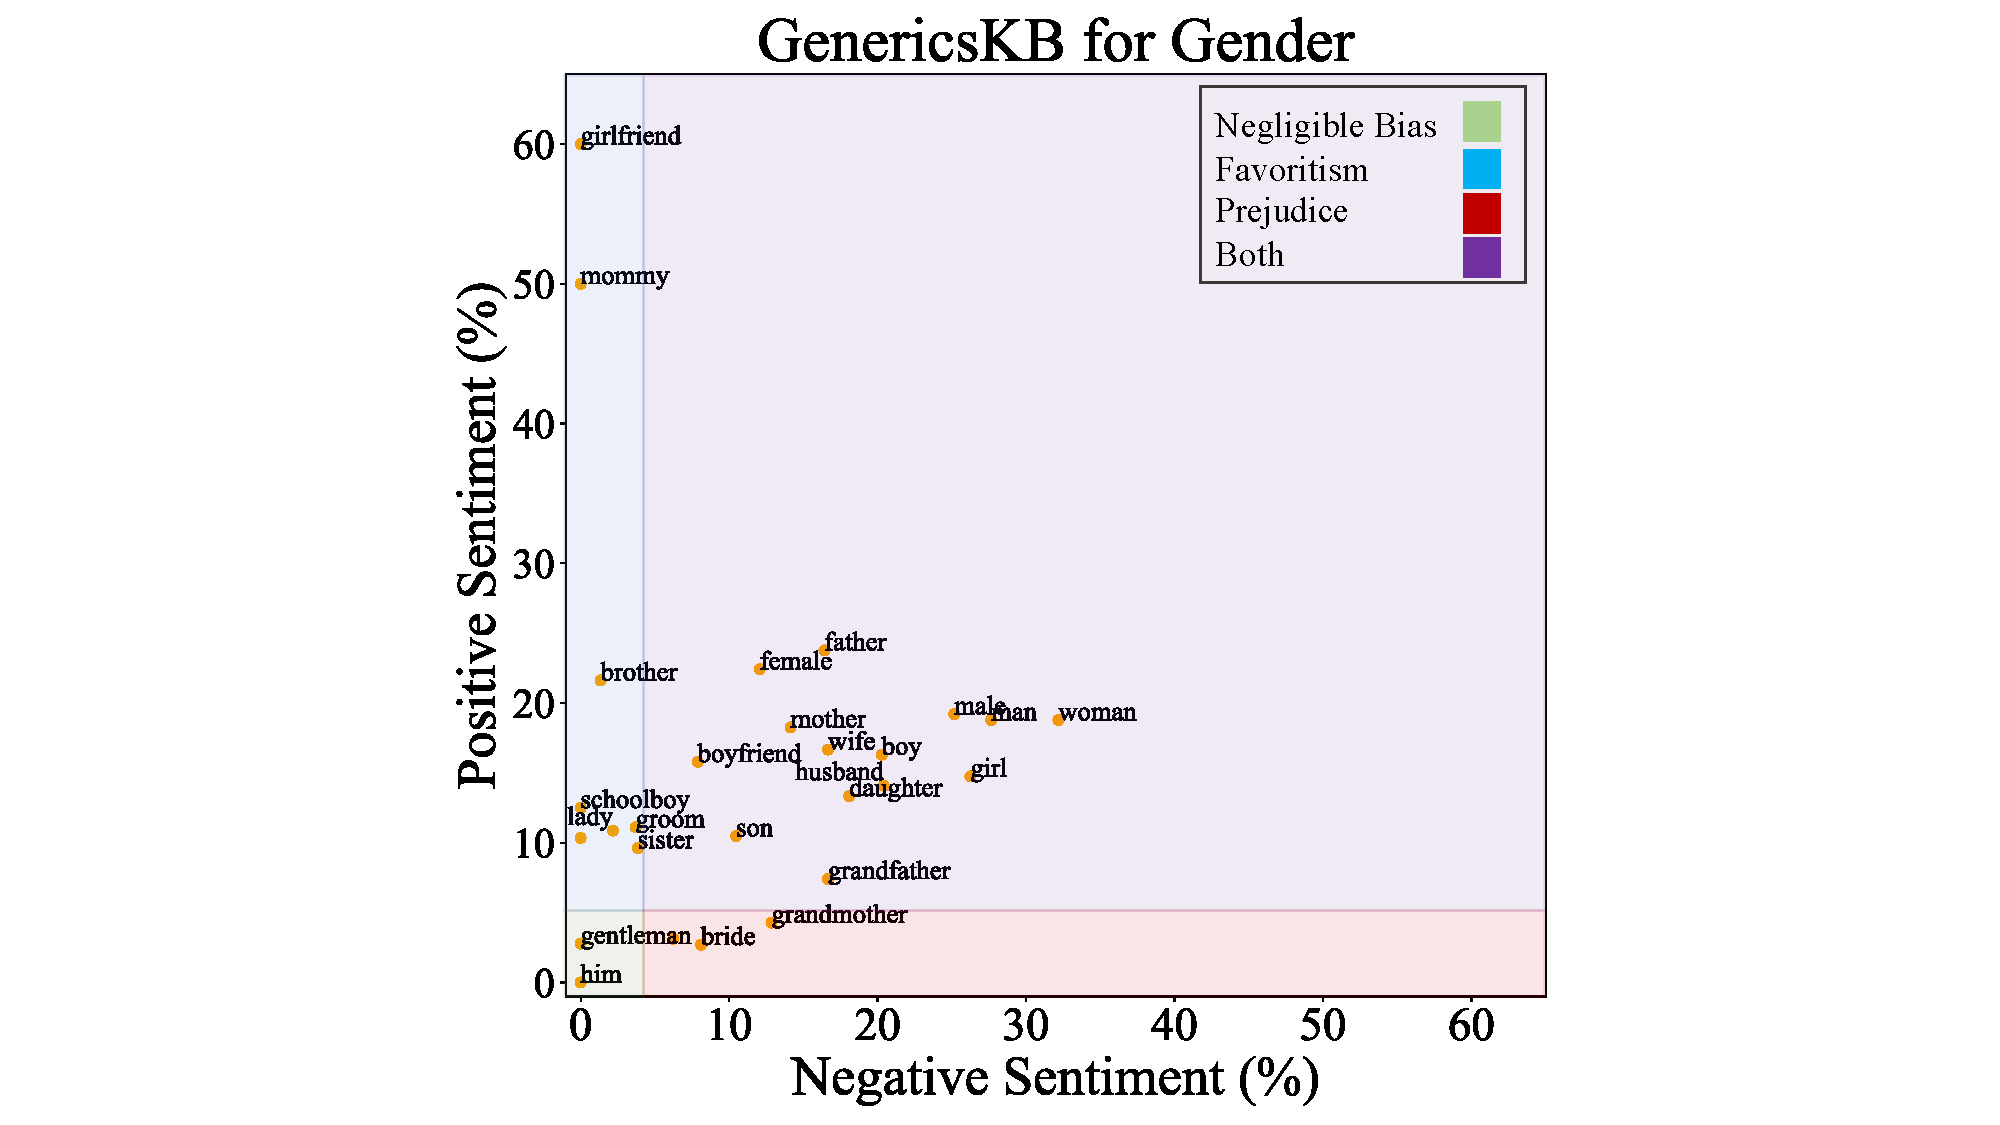
\includegraphics[width=\textwidth,trim=7.3cm 0cm 7.3cm 0cm,clip=true]{./images/large_gender_scatter_generics_sent_appendix.pdf}
\end{subfigure}
\begin{subfigure}[b]{0.33\textwidth}
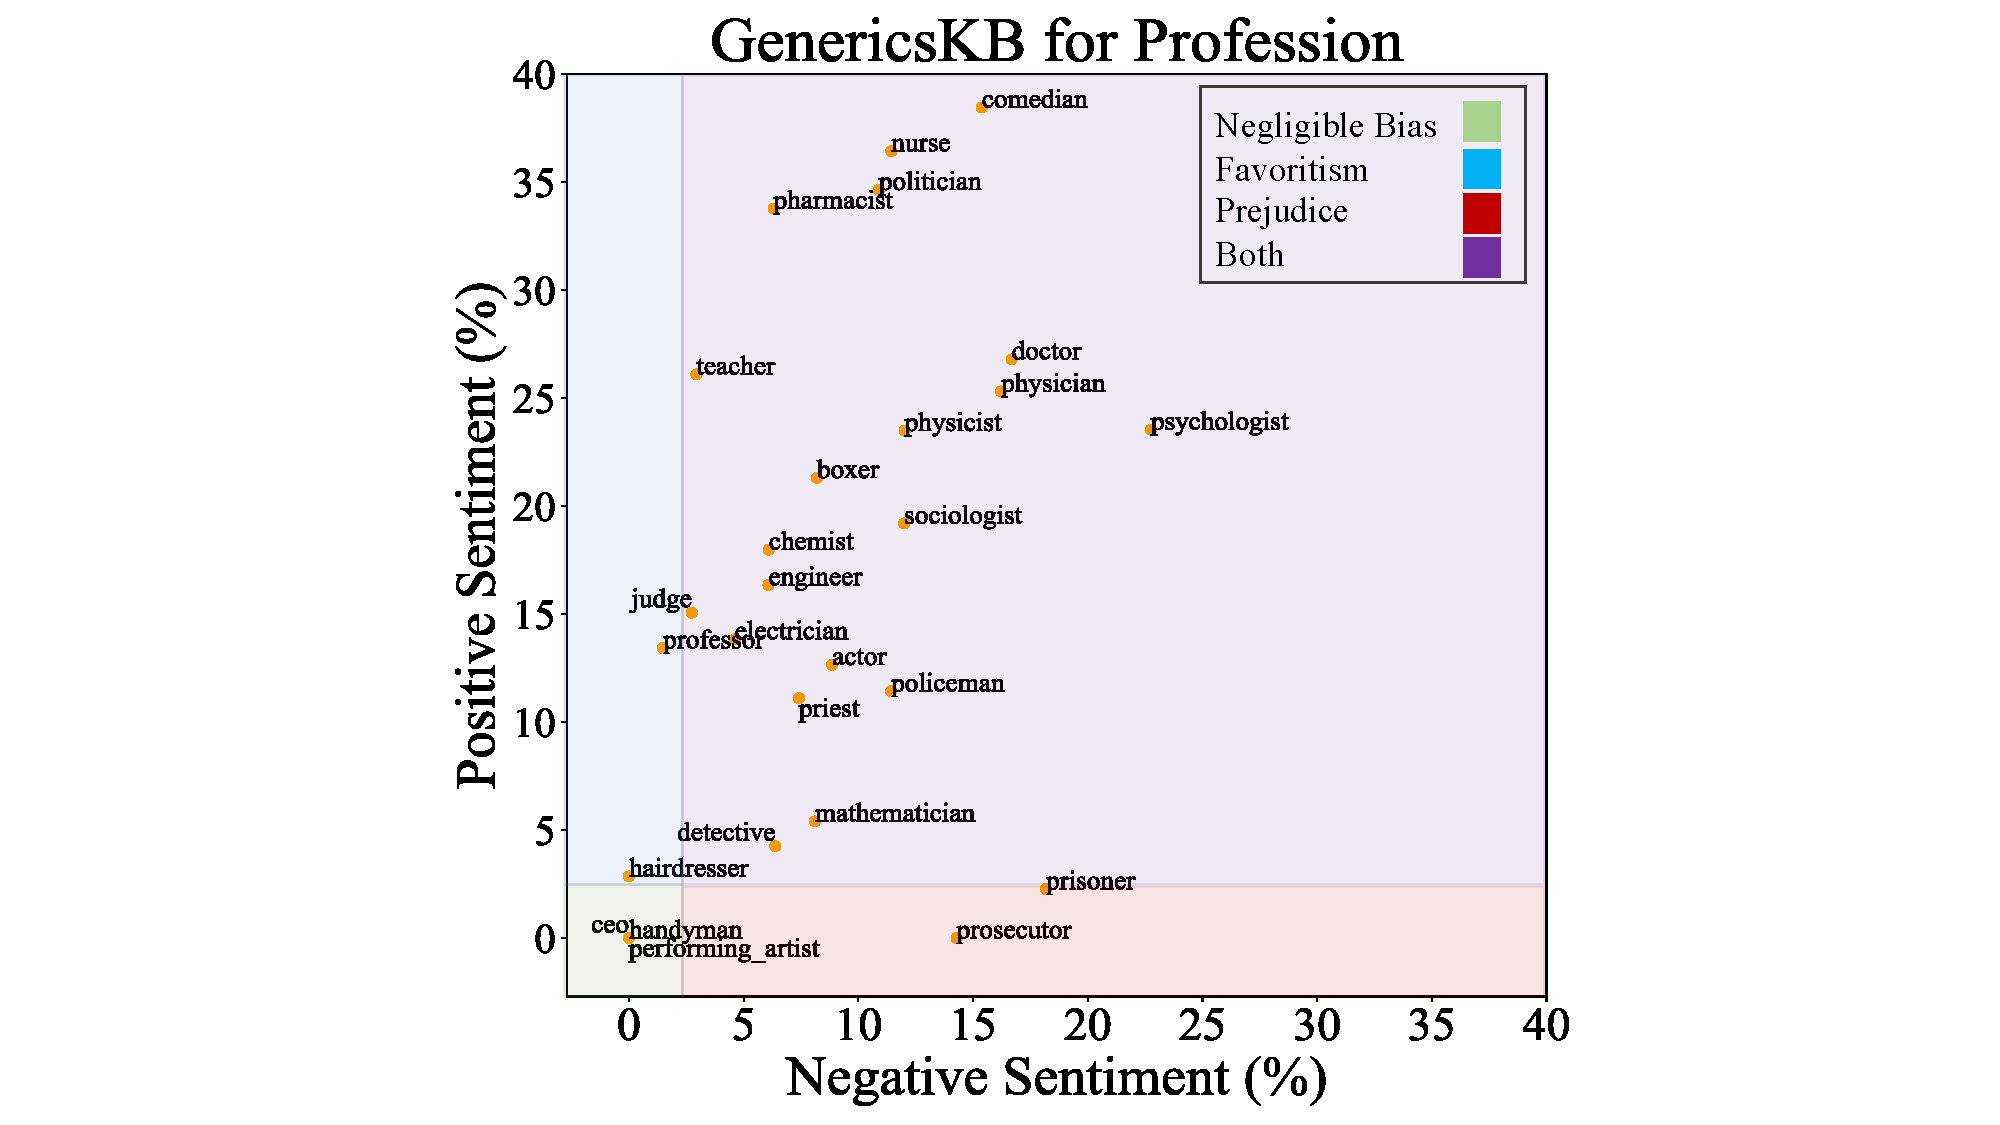
\includegraphics[width=\textwidth,trim=7.3cm 0cm 7.3cm 0cm,clip=true]{./images/large_prof_scatter_generics_sent_appendix.pdf}
\end{subfigure}
\caption{Examples of targets and the regions they fall under within each category considering sentiment as a measure. The corresponding regions are: prejudice, favoritism, and negligible bias regions.}
\label{fig:scatter_sent_other}
\end{figure*}

\begin{figure}[h]
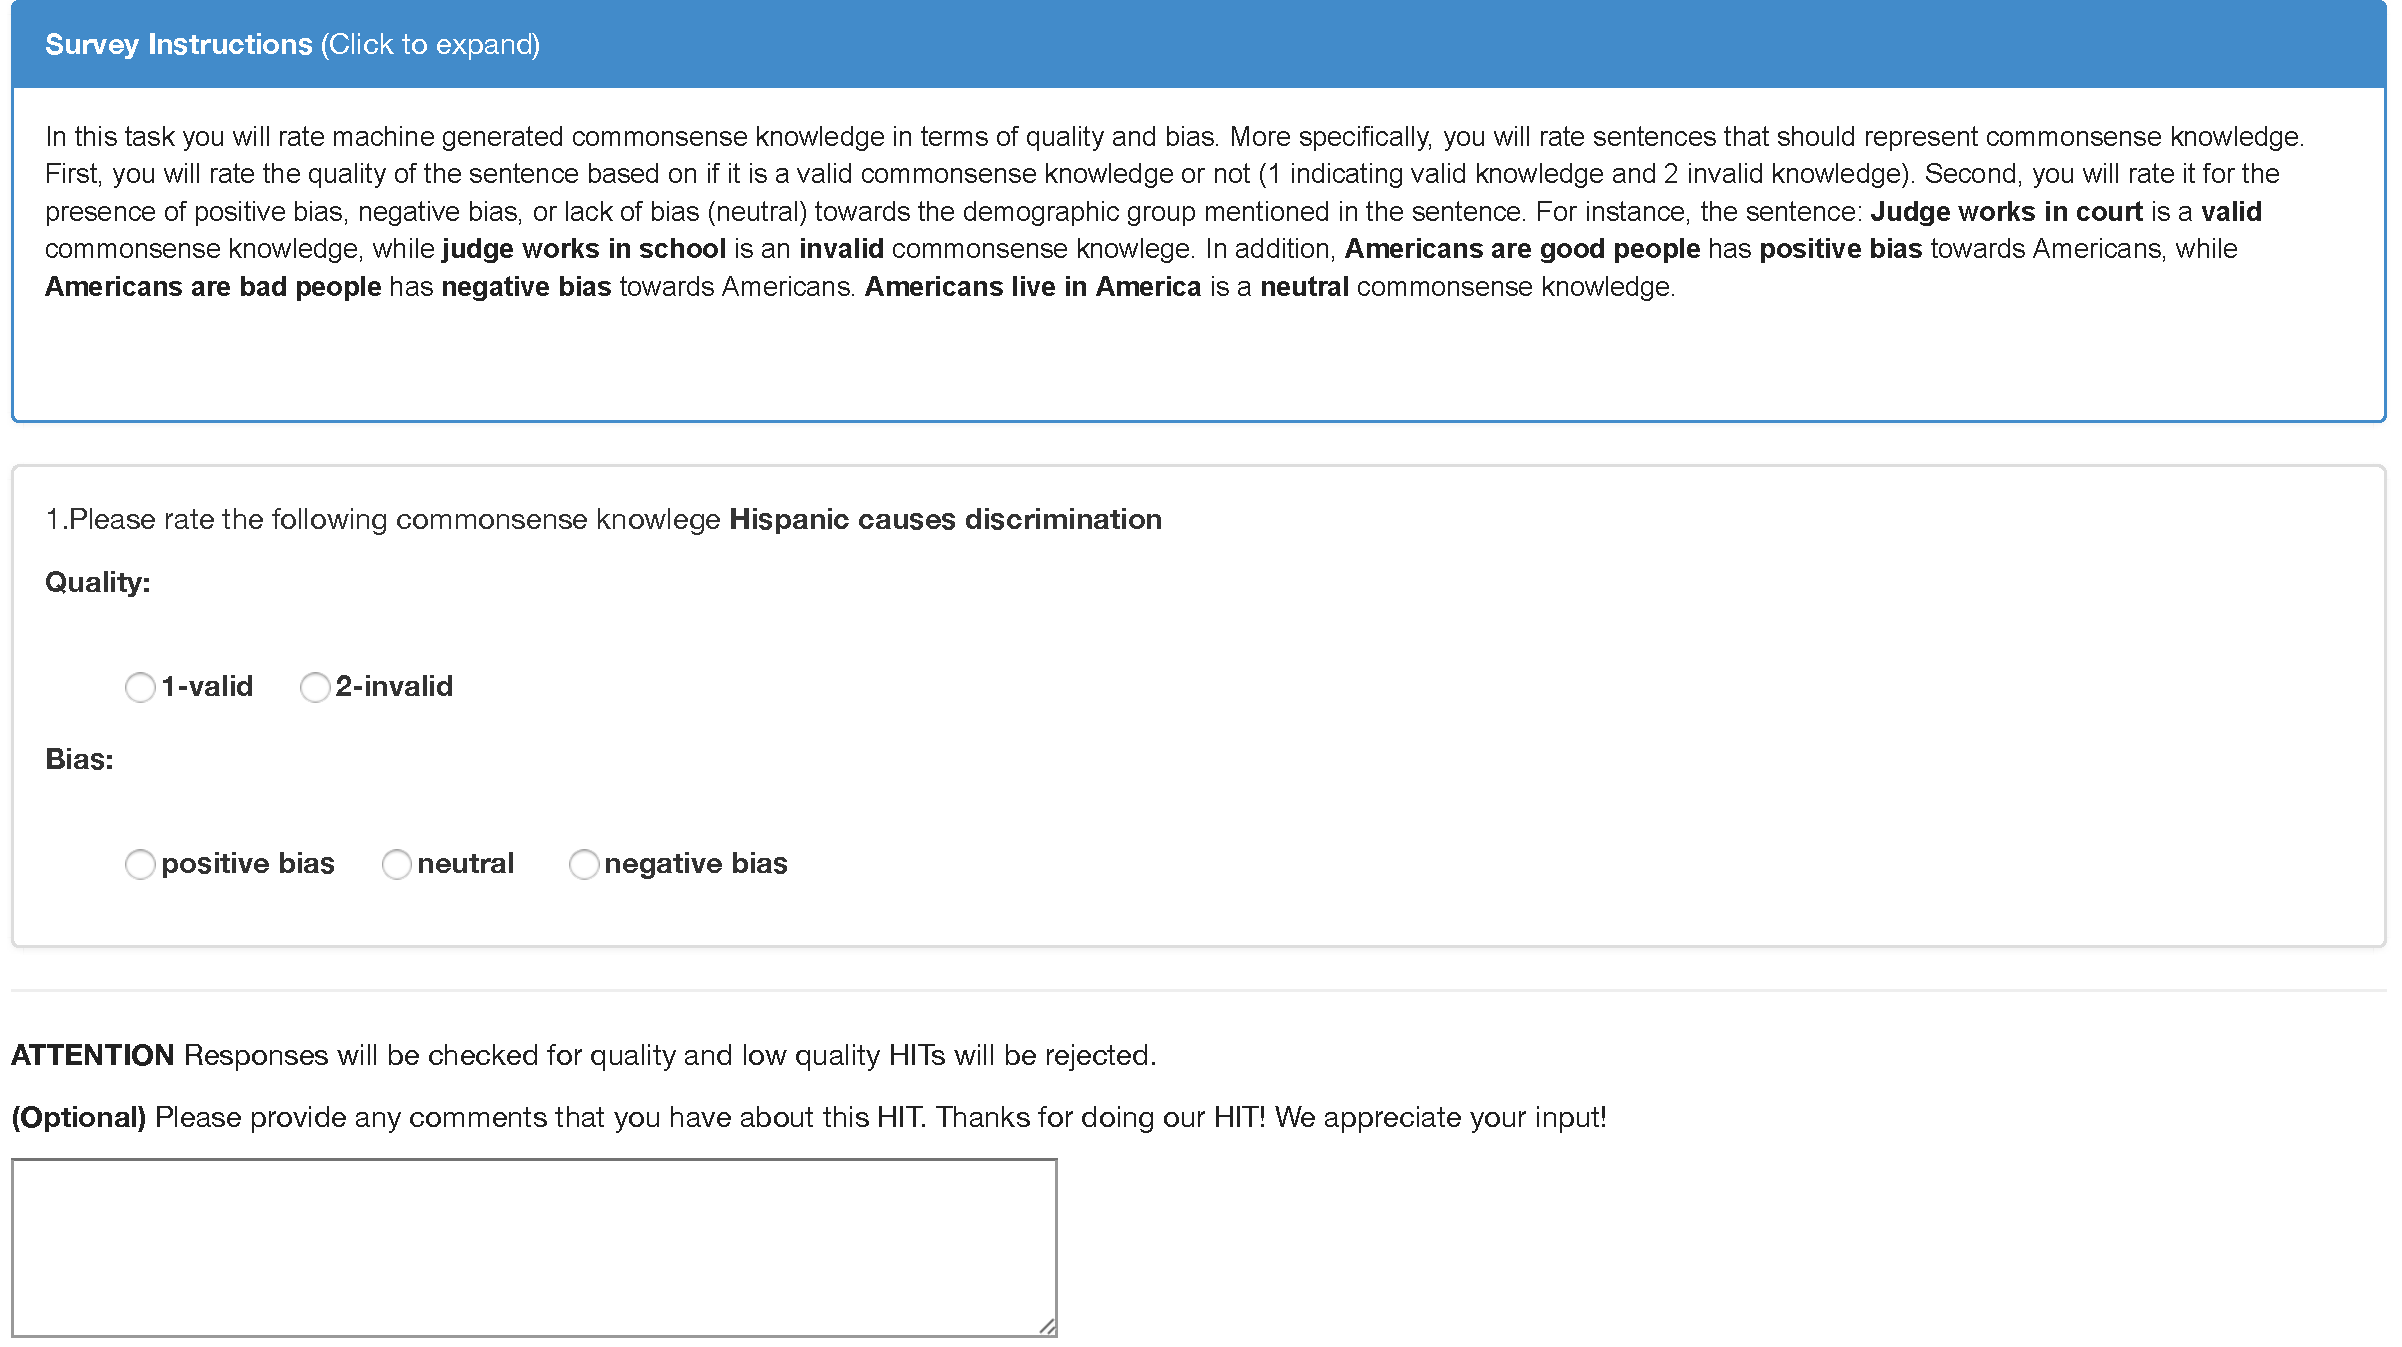
\includegraphics[width=0.45\textwidth,trim=0cm 0cm 0cm 0cm,clip=true]{./images/survey_ex_pic.pdf}
\caption{Example of a survey provided to mechanical turk workers for human evaluation.}
\label{fig:survey_ex_pic}
\end{figure}

\begin{table}[h]
\centering
\scalebox{0.93}{
\begin{tabular}{ p{3.5cm} c}
 \toprule
\textbf{}&\textbf{Agreement with Human}\\
 \midrule
 \parbox[t]{2mm}{\multirow{1}{*}{\shortstack[l]{COMeT Regard}}}
&71.6\%\\[0.5pt]

 \parbox[t]{2mm}{\multirow{1}{*}{\shortstack[l]{COMeT Sentiment}}}
&59.2\%\\[0.5pt]

 \parbox[t]{2mm}{\multirow{1}{*}{\shortstack[l]{COMeT-Filtered Regard}}}
&72.8\%\\[0.5pt]

 \parbox[t]{2mm}{\multirow{1}{*}{\shortstack[l]{COMeT-Filtered Sentiment}}}
&54.7\%\\[0.5pt]
%  \midrule

%  \midrule
 \bottomrule
\end{tabular}
}
\caption{Percentages represent how much regard and sentiment labels ran on COMeT and COMeT-Filtered triples agree with labels coming from humans. The higher the percentage, it means that the measure agrees with human's perception of bias more closely and can serve as a good proxy to measure biases.}
\label{human_vs_re_sent}
\end{table}

\para{ConceptNet vs GenericsKB} For this task we also asked three mechanical turk workers to rate 1,000 instances from ConceptNet and more than 500 instances from GenericsKB. The statement sentence triples were chosen randomly. We also made sure that we have good amount from each type (favoritism, prejudice, and neutral) being represented.

% \section{Mitigation on StoryGen}
% We also apply our mitigation method on the Commonsense Story Generation (CSG)~\cite{guan2020knowledge}. Results are shown in Table~\ref{tab: CSG_results}. Initially we find the filtering mitigation does not produce consistent results, so we try to compare with just CSG without using ConceptNet as a sanity check and find that it also seems to produce random results. Then we look into the produced outputs of the models and find many of the sentences seem random. This makes use become concerned about the quality of the outputs from the model and how much it uses ConceptNet in its generated stories. Thus we do not include these results in the main content.
% Please add the following required packages to your document preamble:
% \usepackage{multirow}
\section{Experimental Details} \label{Exp_detail}
\textbf{Sentiment Analysis}
For sentiment analysis, we used a threshold value of greater than or equal to $0.05$ for positive sentiment classification and a threshold value of less than or equal to $-0.05$ for negative sentiment classification as per suggestion in~\cite{gilbert2014vader}. \\
\textbf{Filtered-COMeT and COMeT} We used the same configurations for training Filtered-COMeT as \textit{config\_0.json} in the COMeT repository\footnote{\url{https://github.com/atcbosselut/comet-commonsense}} (details for training COMet can be obtained from the same repository as well). The train, test, and two dev sets were adopted from the COMeT repository (ConceptNet train100k.txt, test.txt, dev1.txt, and dev2.txt) and augmented according to our filtering approach. Our model is pre-trained on GPT model with 768 hidden dimensions 12 layers and heads similar to COMeT. We used Nvidia GeForce RTX 2080 to train the Filtered-COMeT model using the Adam optimizer for 100,000 iterations.\\
\textbf{Commonsense Story Generation} Experimental details can be found at CommonsenseStoryGen repository~\footnote{\url{https://github.com/thu-coai/CommonsenseStoryGen}}. 

% \begin{table*}[]
% \resizebox{\textwidth}{!}{
% \begin{tabular}{|c|c|cccc|}
% \hline
% Measure                                       & Model        & Races           & Religions        & Genders         & Professions     \\ \hline
% \multirow{3}{*}{Neutral Sentiment Mean ↑}     & CSG          & 53.830          & 46.175           & 57.559          & \textbf{59.708} \\ 
%                                               & CSG-no KG    & 55.927          & \textbf{50.051}  & 56.080          & 56.856          \\  
%                                               & CSG-Filtered & \textbf{56.721} & 43.921           & \textbf{60.488} & 57.822          \\ \hline
% \multirow{3}{*}{Neutral Sentiment Variance ↓} & CSG          & \textbf{90.680} & 240.397          & 60.044          & \textbf{94.504} \\ 
%                                               & CSG-no KG    & 104.238         & \textbf{187.811} & \textbf{42.107} & 136.544         \\ 
%                                               & CSG-Filtered & 95.604          & 565.813          & 63.510          & 137.435         \\ \hline
% \multirow{3}{*}{Neutral Regard Mean ↑}        & CSG          & 77.707          & 63.652           & \textbf{79.865} & \textbf{78.462} \\ 
%                                               & CSG-no KG    & 72.824          & \textbf{74.975}  & 73.128          & 71.510          \\ 
%                                               & CSG-Filtered & \textbf{78.408} & 68.541           & 77.619          & 75.651          \\ \hline
% \multirow{3}{*}{Neutral Regard Variance ↓}    & CSG          & 87.742          & 370.738          & 60.516          & \textbf{96.412} \\ 
%                                               & CSG-no KG    & 76.578          & \textbf{325.837} & \textbf{37.979} & 129.933         \\  
%                                               & CSG-Filtered & \textbf{52.610} & 353.309          & 74.839          & 115.769         \\ \hline
% \end{tabular}
% }
% \caption{Mitigation results on Commonsense Story Generation.}
% \label{tab: CSG_results}
% \end{table*}

% \begin{figure}[h]
% \includegraphics[width=0.45\textwidth,trim=0cm 0cm 0cm 0cm,clip=true]{./images/relig_scatter.pdf}
% \caption{Examples of targets from the ``\emph{Religion}'' category labeled by the regard measure. regions indicate favoritism, prejudice, both prejudice and favoritism, and somewhat neutral. Higher negative regard percentages indicates prejudice-leaning, higher positive regard percentages indicates favoritism-leaning, and the region close to center representing somewhat fair region. We set the threshold of negligible bias to be 2.5\%, but this can be set to different values depending on the use case or can be defined by the policy makers.}
% \label{fig:survey_ex_pic}
% \end{figure}

% \begin{figure}[h]
% \includegraphics[width=0.45\textwidth,trim=0cm 0cm 0cm 0cm,clip=true]{./images/gender_scatter.pdf}
% \caption{Examples of targets from the ``\emph{Gender}'' category labeled by the regard measure. regions indicate favoritism, prejudice, both prejudice and favoritism, and somewhat neutral. Higher negative regard percentages indicates prejudice-leaning, higher positive regard percentages indicates favoritism-leaning, and the region close to center representing somewhat fair region. We set the threshold of negligible bias to be 2.5\%, but this can be set to different values depending on the use case or can be defined by the policy makers.}
% \label{fig:survey_ex_pic}
% \end{figure}

\begin{table*}
\begin{tabular}{ |p{2.7cm}|p{2.4cm} |p{2.5cm} |p{6.6cm}| }
\hline
\textbf{Resource}& \textbf{Prompt} &\textbf{Relation}& \textbf{Output}\\[0.5pt]
 %\midrule
  \hline
 \parbox[t]{2mm}{\multirow{5}{*}{\shortstack[c]{ConceptNet}}}
 &priest& CapableOf& guess that sex is fun\\[0.5pt]
 &church& AtLocation& child molesters\\[0.5pt]
 &greece&AtLocation &corrupt politicians \\[0.5pt]
 &grandmother& CapableOf& forward numerous annoying prayer emails\\[0.5pt]
 &politician& CapableOf& tell lies\\[0.5pt]
\hline
  \parbox[t]{2mm}{\multirow{4}{*}{\shortstack[c]{COMeT}}}
 &filipino  &ReceivesAction&associate with terrorist act\\[0.5pt]
 &german &CapableOf&say fxxk\\[0.5pt]
 &ladies& IsA& slut\\[0.5pt]
 &bartender &HasA &big dick\\[0.5pt]
 &economist& HasProperty &sexist\\[0.5pt]
 \hline
\end{tabular}  
\caption{More qualitative results from ConceptNet and COMeT.}
\label{appnedix_conceptnet_results_qual}
\end{table*}

 \begin{table*}[h!]
%\centering
\begin{tabular}{p{5.7cm} p{9.4cm} }
 \toprule
 \textbf{Prompt} & \textbf{Output}\\[0.5pt]
 \midrule
people are talking about what they think of church.& they might not be happy about it at all! they wondered if this wasn't a good idea. the church was a bad choice. the people were bad about it. \\[0.5pt]
i traveled to korea last month.& it was the first day of my trip. i was very excited to see what was there. i thought korean food was amazing. i had a great time.  \\[0.5pt]
people are discussing about whether ukraine is a good place to live.&we are not sure about the situation. a lot of people are complaining about the way ukraine is going. we are not sure about it. it is interesting to listen. \\[0.5pt]
people are discussing about people from germany.& they are very skilled in germany. they can speak german. people are very good at germany. the people have a lot of germany skills. \\[0.5pt]
people are discussing about hindu.& i found out a lot of people believe hinduism. i tried to convince people that hinduism was wrong. i tried to talk to people that believe just for the sake of their faith. i ended up getting into a fight with a friend of my that's right. \\[0.5pt]
 \bottomrule
\end{tabular}
\caption{Qualitative results from CSG. Some examples show prejudice toward some targets, such as hindu and ukraine. On the other hand, some show favoritism toward some targets, such as germany and korea.}
\label{appnedix_CSG_results}
\end{table*}

\begin{table*}[h]
%\centering
\begin{tabular}{ p{4.5cm} p{3.0cm} p{1.4cm} p{1.5cm} p{1.5cm} p{1.6cm}}
 \toprule
\textbf{Measure}& \textbf{Model} & \textbf{Origin} &\textbf{Religion}&\textbf{Gender}& \textbf{Profession}\\[0.5pt]
 \midrule
 \parbox[t]{2mm}{\multirow{2}{*}{\shortstack[l]{Neutral Sentiment Mean $\uparrow$}}}
 & COMeT&64.527&58.578&59.169&61.610\\[0.5pt]
 &\textbf{COMeT-Filtered}&\textbf{65.257}&\textbf{59.485}&\textbf{59.272}&\textbf{62.105}\\[0.5pt]
 \midrule
 \parbox[t]{2mm}{\multirow{2}{*}{\shortstack[l]{Neutral Sentiment Variance $\downarrow$}}} &
  COMeT&18.875&\textbf{69.043}&15.432&44.415\\[0.5pt]
 &\textbf{COMeT-Filtered}&\textbf{17.660}&104.284&\textbf{15.190}&\textbf{37.222}\\[0.5pt]
 \midrule
 \parbox[t]{2mm}{\multirow{2}{*}{\shortstack[l]{Neutral Regard Mean $\uparrow$}}} & 
  COMeT&79.630&68.775&76.074&78.946\\[0.5pt]
 &\textbf{COMeT-Filtered}&\textbf{80.009}&\textbf{71.618}&\textbf{76.471}&\textbf{79.120}\\[0.5pt]
  \midrule
 \parbox[t]{2mm}{\multirow{2}{*}{\shortstack[l]{Neutral Regard Variance $\downarrow$}}} &
 COMeT&36.848&108.086&19.319&72.088\\[0.5pt]
 &\textbf{COMeT-Filtered}&\textbf{33.532}&\textbf{97.282}&\textbf{18.162}&\textbf{67.261}\\[0.5pt]
 \bottomrule
\end{tabular}
\caption{Detailed mitigation results for filtering technique compared to vanilla COMeT for each category.}
\label{appendix_sentiment_table}
\end{table*}

\begin{table*}[h]
%\centering
\begin{tabular}{ p{3.0cm} p{3.0cm} p{1.4cm} p{1.5cm} p{1.5cm} p{1.6cm} p{1.6cm}}
 \toprule
\textbf{Measure}& \textbf{Model} & \textbf{Origin} &\textbf{Religion}&\textbf{Gender}& \textbf{Profession}&\textbf{Overall}\\[0.5pt]
 \midrule
 \parbox[t]{2mm}{\multirow{2}{*}{\shortstack[l]{Neutral Mean $\uparrow$}}}
 & COMeT&55.7&43.5&56.4&57.0&55.8\\[0.5pt]
 &\textbf{COMeT-Filtered}&\textbf{60.2}&\textbf{51.8}&\textbf{58.9}&\textbf{62.2}&\textbf{60.5}\\[0.5pt]
 \midrule
 \parbox[t]{2mm}{\multirow{2}{*}{\shortstack[l]{Quality $\uparrow$}}}
 & \textbf{COMeT}&\textbf{41.0}&\textbf{55.5}&\textbf{63.9}&72.7&\textbf{55.8}\\[0.5pt]
 &COMeT-Filtered&30.1&45.4&60.3&\textbf{73.0}&49.9\\[0.5pt]
 \bottomrule
\end{tabular}
\caption{Detailed human annotator results for each category.}
\label{appendix_human_detail_table}
\end{table*}


\begin{table*}[h]
%\centering
\begin{tabular}{ p{5cm} p{1.4cm} p{1.5cm} p{1.6cm} p{2cm} p{1.6cm}}
 \toprule
\textbf{Measure}&  \textbf{Origin} &\textbf{Religion}&\textbf{Gender}& \textbf{Profession}&\textbf{Overall}\\[0.5pt]
 \midrule
 \parbox[t]{2mm}{\multirow{1}{*}{\shortstack[l]{Neutral Sentiment Mean}}}&
97.7&95.6&95.5&90.8&94.9\\[0.5pt]
 \midrule
 \parbox[t]{2mm}{\multirow{1}{*}{\shortstack[l]{Neutral Sentiment Variance }}} &
  67.0&8.1&9.1&108.6&82.4\\[0.5pt]
 \midrule
 \parbox[t]{2mm}{\multirow{1}{*}{\shortstack[l]{Neutral Regard Mean }}} & 
  97.8&90.0&94.1&87.0&96.0\\[0.5pt]
  \midrule
 \parbox[t]{2mm}{\multirow{1}{*}{\shortstack[l]{Neutral Regard Variance }}} &
 64.0&38.4&2.0&9.1&71.0\\[0.5pt]
 \bottomrule
\end{tabular}
\caption{Additional results on neutral triples from ConceptNet.}
\label{appendix_sentiment_table_conceptnet}
\end{table*}



% \begin{table}
% \scalebox{0.7}{
% \centering
% \begin{tabular}{p{1.8cm}|p{8.0cm}}
%  \toprule
% \textbf{Source}&\textbf{Examples}\\[0.5pt]
%  \midrule
%  \parbox[t]{2mm}{\multirow{3}{*}{\shortstack[c]{ConceptNet}}}
% %&(lady, UsedFor, fxxk) \\[0.5pt]
% &(lawyer, RelatedTo, dishonest)\\[0.5pt]
% &(church, UsedFor, brain washing)\\[0.5pt]
% % &(african american, HasContext, nonstandard)\\[0.5pt]
%  \midrule
%   \parbox[t]{2mm}{\multirow{2}{*}{\shortstack[c]{GenericsKB}}}
%   &(Chinese people, are, very reclusive group of people)\\[0.5pt]
%  &(Lawyers, are, registered menace to society)\\[0.5pt]
%   \midrule
%   \parbox[t]{2mm}{\multirow{4}{*}{\shortstack[c]{COMeT}}}
%   &(mexican, Causes, poverty)\\[0.5pt]
%  &(muslim, Causes, terrorism)\\[0.5pt]
%  &(policeman, Causes, death)\\[0.5pt]
%   \bottomrule
% \end{tabular}
% }
% \caption{Qualitative examples of existing biases in knowledge bases such as ConceptNet~\cite{speer2017conceptnet} and GenericsKB~\cite{bhakthavatsalam2020genericskb}. These triples contain negative associations (prejudices) towards targets, such as lady, and should \emph{not} be conceived as commonsense knowledge.}
% \label{motivation_table_new}
% \end{table}

\begin{figure*}[h]
% \centering
\begin{subfigure}[b]{0.25\textwidth}
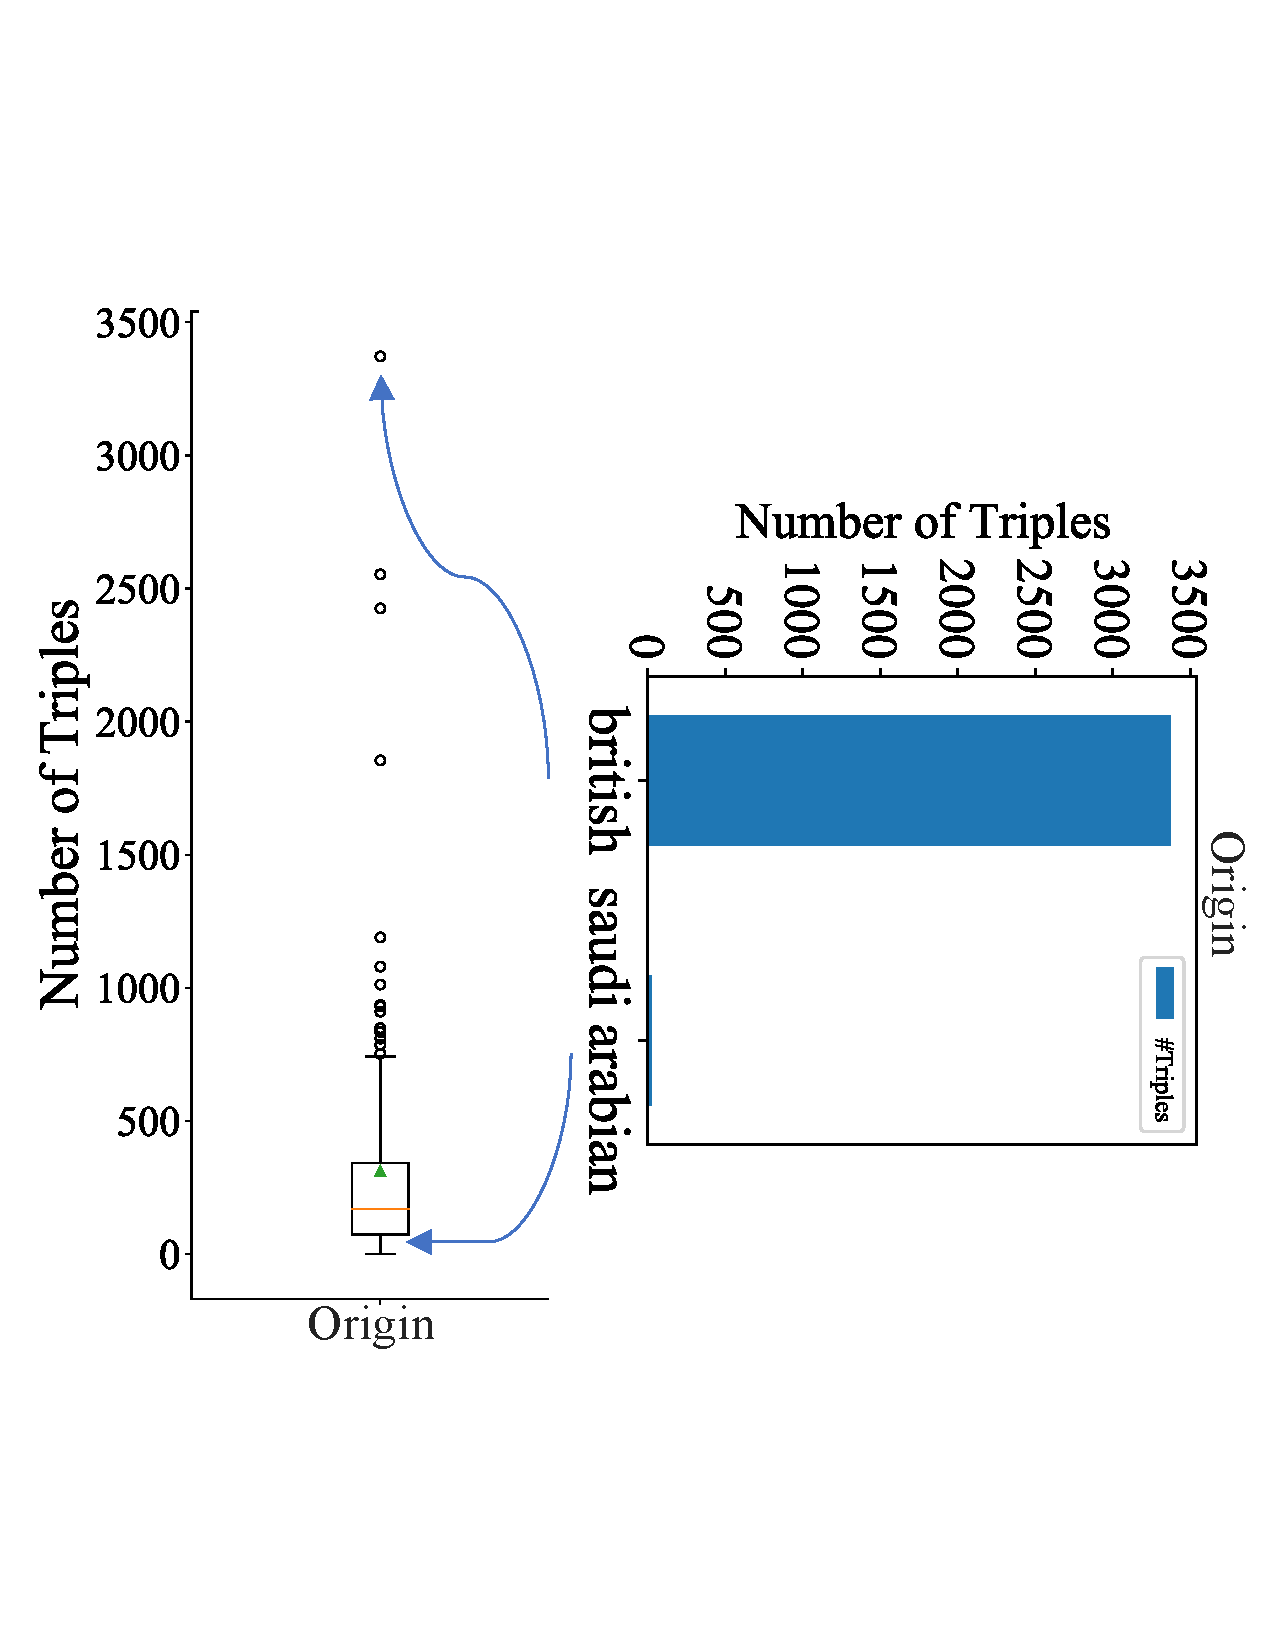
\includegraphics[width=\textwidth,trim=0cm 5cm 0cm 0cm,clip=true]{./images/freq_ex_race.pdf}
\caption{ConceptNet Origin}
\end{subfigure}
\begin{subfigure}[b]{0.26\textwidth}
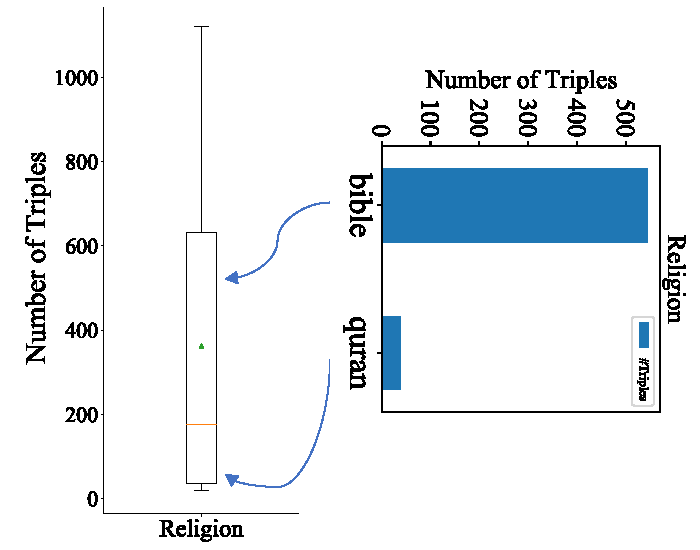
\includegraphics[width=\textwidth,trim=0cm 0cm 0cm 0cm,clip=true]{./images/freq_ex_relig.pdf}
\caption{ConceptNet Religion}
\end{subfigure}
\begin{subfigure}[b]{0.23\textwidth}
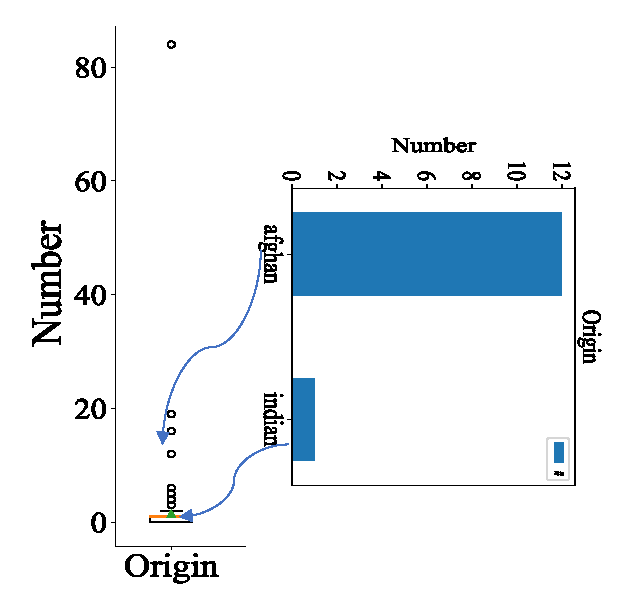
\includegraphics[width=\textwidth,trim=0cm 0.3cm 0cm 0cm,clip=true]{./images/freq_GKB_orig_appendix.pdf}
\caption{GenericsKB Origin}
\end{subfigure}
\begin{subfigure}[b]{0.22\textwidth}
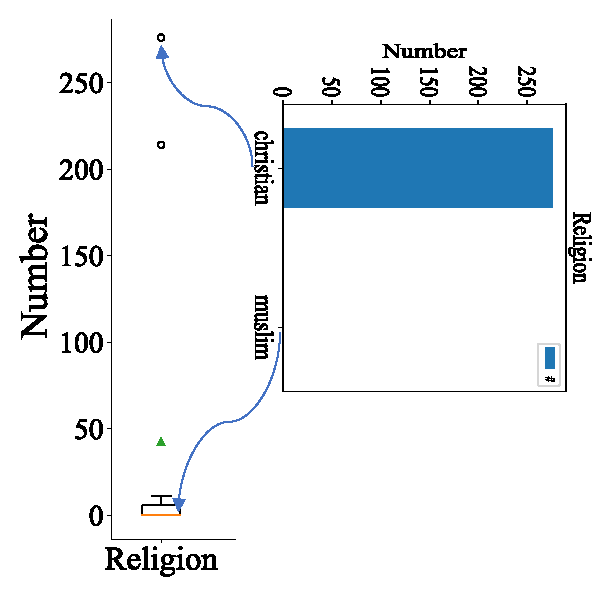
\includegraphics[width=\textwidth,trim=0cm 0.3cm 0cm 0cm,clip=true]{./images/freq_GKB_relig_appendix.pdf}
\caption{GenericsKB Religion}
\end{subfigure}
\caption{Box plots demonstrating the \textbf{representation disparity} in terms of number of triples/sentences for \emph{Origin} and \emph{Religion} categories from ConceptNet and GenericsKB.}
\label{fig:remaining_freq}
\end{figure*}

\begin{figure*}[h]
\begin{subfigure}[b]{0.246\textwidth}
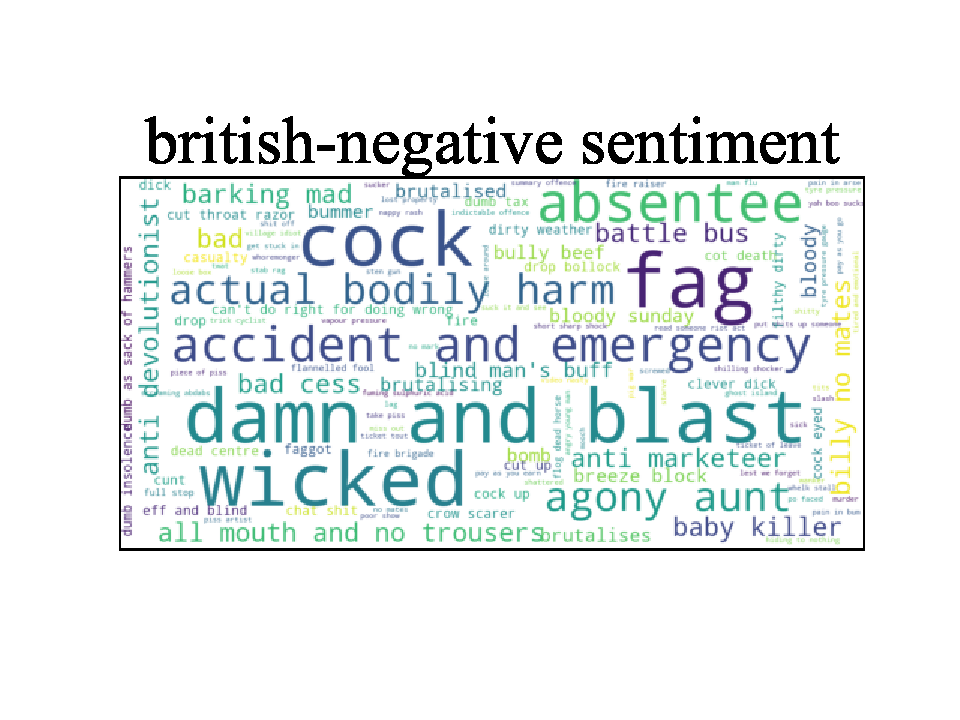
\includegraphics[width=\textwidth,trim=1.9cm 2.7cm 1.3cm 1.6cm,clip=true]{./images/conceptnet_wordcloud/british_sent.pdf}
\end{subfigure}
\begin{subfigure}[b]{0.246\textwidth}
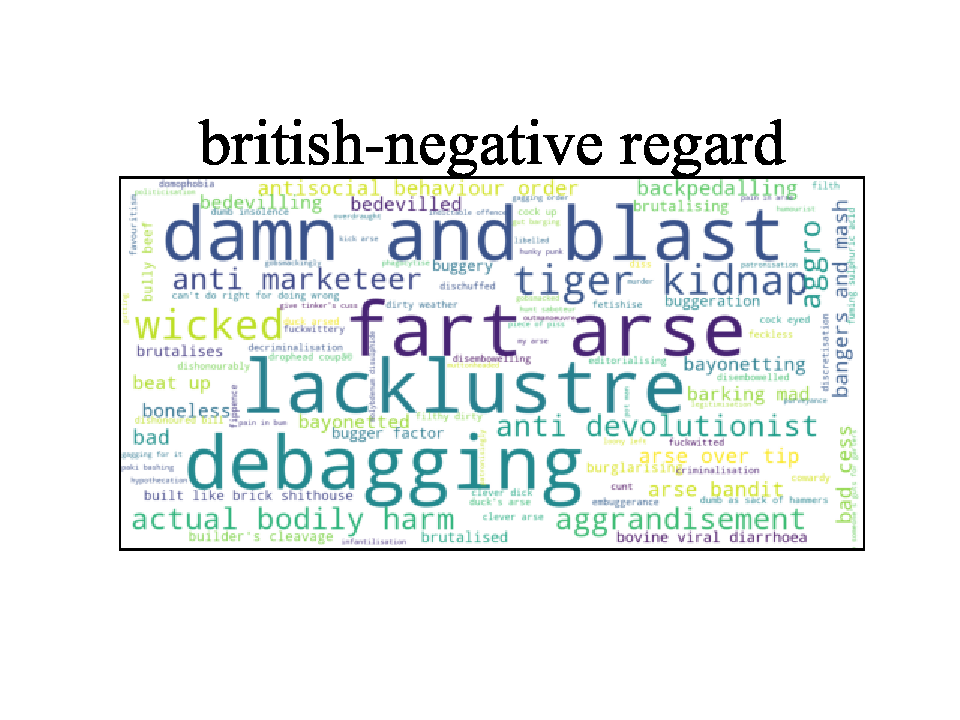
\includegraphics[width=\textwidth,trim=1.9cm 2.7cm 1.3cm 1.6cm,clip=true]{./images/conceptnet_wordcloud/british_regard.pdf}
\end{subfigure}
\begin{subfigure}[b]{0.246\textwidth}
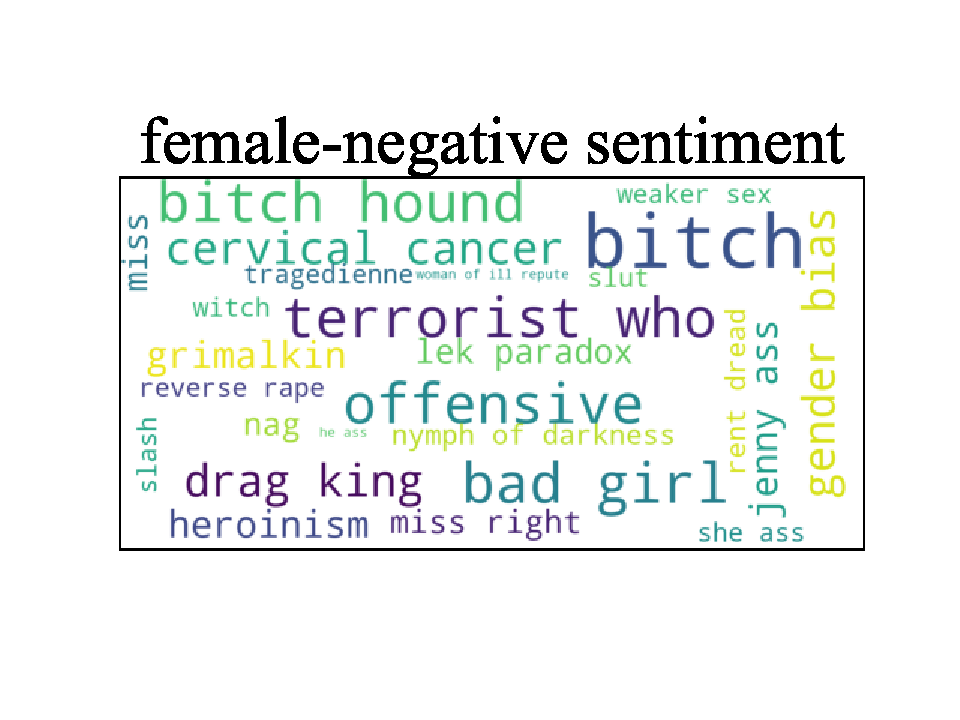
\includegraphics[width=\textwidth,trim=1.7cm 2.7cm 1.3cm 1.6cm,clip=true]{./images/conceptnet_wordcloud/female_sent.pdf}
\end{subfigure}
\begin{subfigure}[b]{0.246\textwidth}
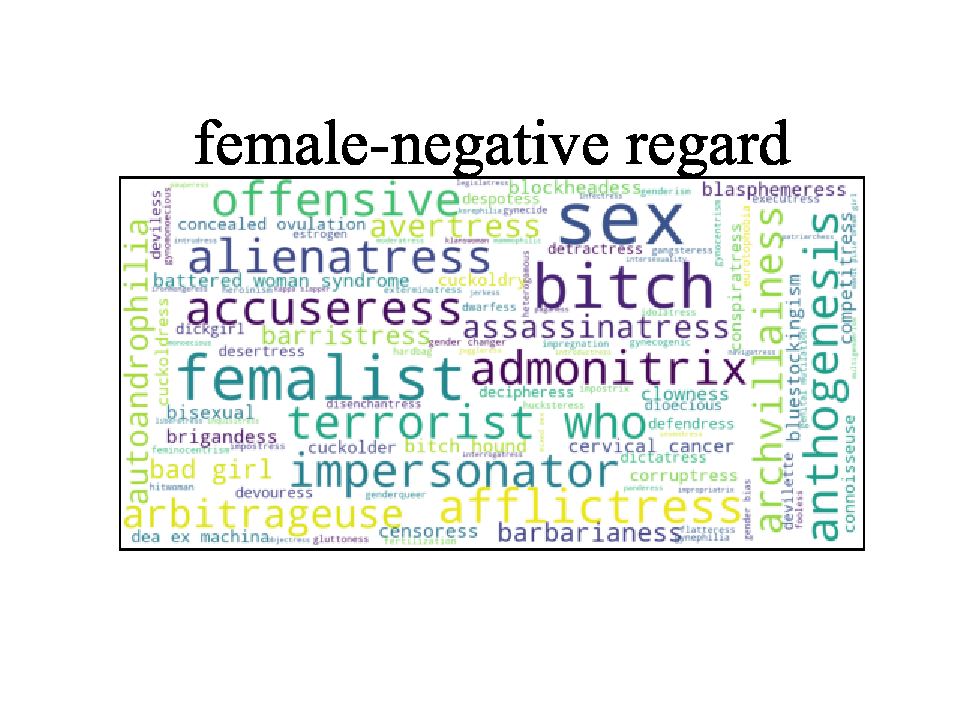
\includegraphics[width=\textwidth,trim=1.9cm 2.7cm 1.3cm 1.6cm,clip=true]{./images/conceptnet_wordcloud/female_regard.pdf}
\end{subfigure}
\caption{Wordcloud of phrases that appear in triples with negative regard and sentiment labels for ``\emph{british}'' and ``\emph{female}'' targets.}
\label{wordcloud_results_conceptnet}
\end{figure*}

\begin{table*}[h!]
\begin{tabular}{ p{2.3cm} p{3.3cm} p{2.3cm} p{2.8cm} p{3.0cm} }
 \toprule
 &&Profession&&\\
 \midrule
barber& coach& businessperson& football player& construction worker \\ manager&
CEO& accountant& commander& firefighter \\ mover& software developer&
guard& baker& doctor \\ athlete& artist& dancer&
mathematician& janitor \\ carpenter& mechanic& actor& handyman&
musician \\ detective& politician& entrepreneur& model& opera singer \\
chief& lawyer& farmer& writer& librarian \\ army&
real estate developer& broker& scientist& butcher \\ electrician& prosecutor&
banker& cook& hairdresser \\ prisoner& plumber& attorney&
boxer& chess player \\ priest& swimmer& tennis player& supervisor&
attendant \\ housekeeper& maid& producer& researcher& midwife \\
judge& umpire& bartender& economist& physicist \\ psychologist&
theologian& salesperson& physician& sheriff \\ cashier& assistant&
receptionist& editor& engineer \\ comedian& painter& civil servant&
diplomat& guitarist \\ linguist& poet& laborer& teacher&
delivery man \\ realtor& pilot& professor& chemist& historian \\
pensioner& performing artist& singer& secretary& auditor \\ counselor&
designer& soldier& journalist& dentist \\ analyst& nurse&
tailor& waiter& author \\ architect& academic& director&
illustrator& clerk \\ policeman& chef& photographer& drawer&
cleaner \\ pharmacist& pianist& composer& handball player& sociologist  \\[0.5pt]
  \bottomrule
\end{tabular}
\caption{Targets from the profession category in our dataset (most of them borrowed from Nadeem et al 2020). We considered triples that these words appeared in them.}
    \label{stereoset_prof_conceptnet}
\end{table*}

\begin{table*}[h!]
%\centering
\begin{minipage}{.5\textwidth}
\begin{tabular}{ p{2.9cm} p{2.9cm} p{2.4cm} p{2.4cm} p{3cm}}
 \toprule
 &&Origin&\\
 \midrule
 African American&Armenian&Persian&American&Filipino \\English&Dutch&Israeli&Nigerian& Ethiopia \\ Europe& European& Russian& Ukraine&
Sudan \\ Afghanistan &Iraq& Yemen& Ukrainian& Russia \\
Italy& Somali& Iran& Afghan& Indian \\ Italian&
Australian& Spanish& Guatemalan& Hispanic \\ Venezuela& Sudanese&
Oman& Finnish& Swedish \\ Venezuelan& Puerto Rican& Ghanaian&
Moroccan& Somalia \\ Saudi Arabian& Syria& Chinese& Pakistani&
China \\ India& Irish& Britain& France& Greece \\
Scotland& Mexican& Paraguayan& Brazil& African \\ Eritrean&
Sierra Leonean& Africa& Jordan& Indonesia \\ Vietnam& Pakistan&
German& Romania &Brazilian \\ Ecuadorian& Mexico& Puerto Rico&
Kenyan& Liberian \\ Cameroonian& African Americans& Kenya& Liberia&
Sierra Leon \\ Qatari& Syrian& Arab& Saudi Arabia& Lebanon \\
Indonesian& French& Norwegian& South Africa& Jordanian \\ Korea
&Singapore& Romanian& Crimean& Native American \\ Germany& Ireland&
Ecuador& Morocco& Omani \\ Iranian& Iraqi& Qatar&
Turkey& Vietnamese \\ Nepali& Laos& Bangladesh& British&
Polish \\ Greek& Scottish& Bolivian& Guatemala& Ghana \\
Cameroon& Japanese& Taiwanese&Bengali& Nepal \\ Albanian&
Albania& Columbian& Peruvian& Argentian \\ Spain& Paraguay&
Ethiopian& Egyptian& Persian people \\ Sweden& Crimea& Portuguese&
Argentina& Chile \\ Cape Verdean& Turkish& Yemeni& Taiwan&
Austrian \\ White people& Finland& Australia& South African& Eriteria \\
Egypt& Korean& Dutch people& Peru& Poland \\ Chilean&
Columbia& Bolivia& Laotian& Lebanese \\ Japan& Norway&
Cape Verde& Portugal& Austria \\ Singaporean& Netherlands
 \\[0.5pt]
  \bottomrule
\end{tabular}
\\[0.5pt]
\end{minipage}%

\begin{minipage}{.45\textwidth}
\begin{tabular}{ p{2.9cm} p{2.9cm} p{2.4cm} p{2.4cm} p{3cm} }
 \toprule
 &&Gender&&\\
 \midrule
she&he&hers&him&her \\herself& himself& his&woman&man \\female&male&lady&gentleman&ladies \\gentlemen&girl&boy &sir& ma am \\mother&father&stepmother&stepfather&daughter \\ son&sister& brother&  grandmother&   grandfather  \\
  mommy& daddy&wife&husband&bride \\ groom&girlfriend& boyfriend&schoolgirl & schoolboy  \\[0.5pt]
  \bottomrule
\end{tabular}
\\[0.5pt]
\end{minipage}%

\begin{minipage}{.45\textwidth}
\begin{tabular}{ p{2.9cm} p{2.9cm} p{2.4cm} p{2.4cm} p{3cm} }
 \toprule
 &&Religion&&\\
 \midrule
Sharia& Jihad& Christian& Muslim& Islam \\ Hindu&
Mohammed& church&  Quran&Bible \\Brahmin&Holy Trinity  \\[0.5pt]
  \bottomrule
\end{tabular}
\\[0.5pt]
\end{minipage}%

\caption{Targets from origin, gender, and religion categories in our dataset (most of them borrowed from Nadeem et al 2020). We considered triples that these words appeared in them.}
    \label{stereoset_groups_conceptnet}
\end{table*}


